% vim: tw=80

\chapter{Constraints on PDFs and Determination of the Strong Coupling Constant}
\label{sec:pdf_constraints}

In many precision measurements at the LHC, the proton PDFs are an essential
ingredient. As the PDFs cannot be calculated from perturbative QCD, they are
derived from fits to experimental data of collider and fixed-target experiments.
The precise DIS data from the HERA collider provides the base data sets as they
cover most of the kinematic phase space. By adding more data from different
experiments, the precision on the PDFs can be improved. To study the the
constraints of the triple-differential dijet cross section on the PDFs, a
combined fit of the dijet data and the DIS data from HERA is performed.

\section{Correlation between dijet cross section and PDFs}
\label{sec:pdf_sensitivity}

To illustrate the phase space regions in which the triple-differential dijet
cross section has an impact on the the PDFs, the correlation between the
cross section $\sigma(Q)$ and the PDF $xf(x,Q^2)$ for any parton flavor~$f$ can
be calculated. The PDF sets of the NNPDF collaboration are an ensemble of
replicas $i$, which sample variations in the PDF parameter space within the
PDF's uncertainties. The correlation coefficient $\varrho_f(x,Q)$ between the cross section and the PDF for
flavour~$f$ at a point $(x,Q)$ can be computed by evaluating means and standard
deviations from an ensemble of $N$ replicas as

\begin{equation}
  \varrho_f (x,Q) =
  \frac{N}{(N-1)} \frac{%
    \langle \sigma(Q)_i \cdot xf(x,Q^2)_i \rangle -
    \langle \sigma(Q)_i \rangle \cdot
    \langle xf(x,Q^2)_i \rangle}
  {\Delta_{\sigma(Q)} \Delta_{xf(x,Q^2)}}\,.
\end{equation}

where angular brackets denote the averaging over all replicas, and
$\Delta_{\sigma(Q)}$ and $\Delta_{xf(x,Q^2)}$ are the standard deviations of the
dijet cross section or of the PDF with flavour $f$, respectively.
Fig.~\ref{fig:correlation_pdf_xs_gqq} presents the correlation coefficient
between the dijet cross section and the gluon, u valence quark, and d
valence quark PDFs in the proton for the most central bin with low \ystar and
low \yboost values and the bin containing boosted dijet events ($2 \leq \yboost
< 3$).

\begin{figure}[p]
  \centering
  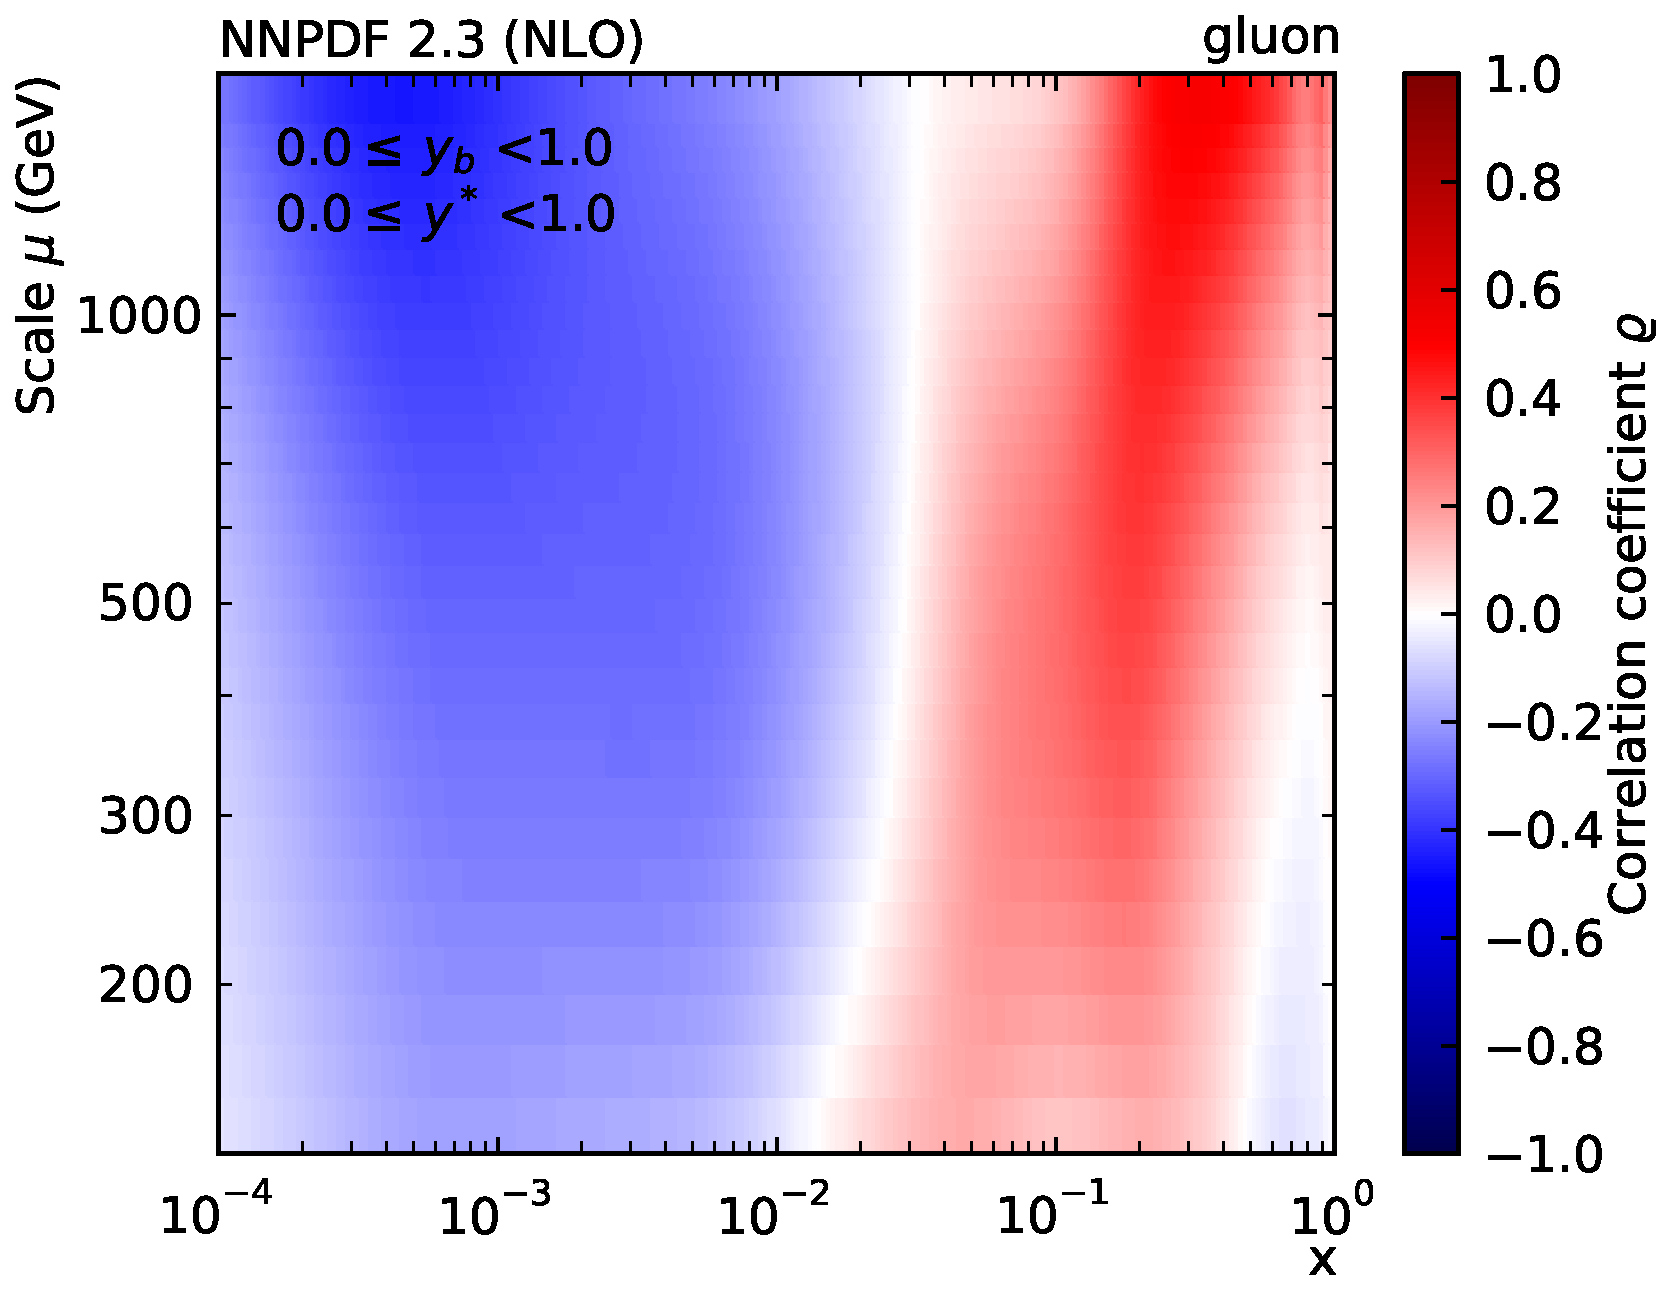
\includegraphics[width=0.49\textwidth]{figures/pdf_constraints/corr_PTMAXEXPYS_YBYS_NLO_FINALBINS_NNPDF23_gluon_ys0_0yb0_0_cl.pdf}\hfill%
  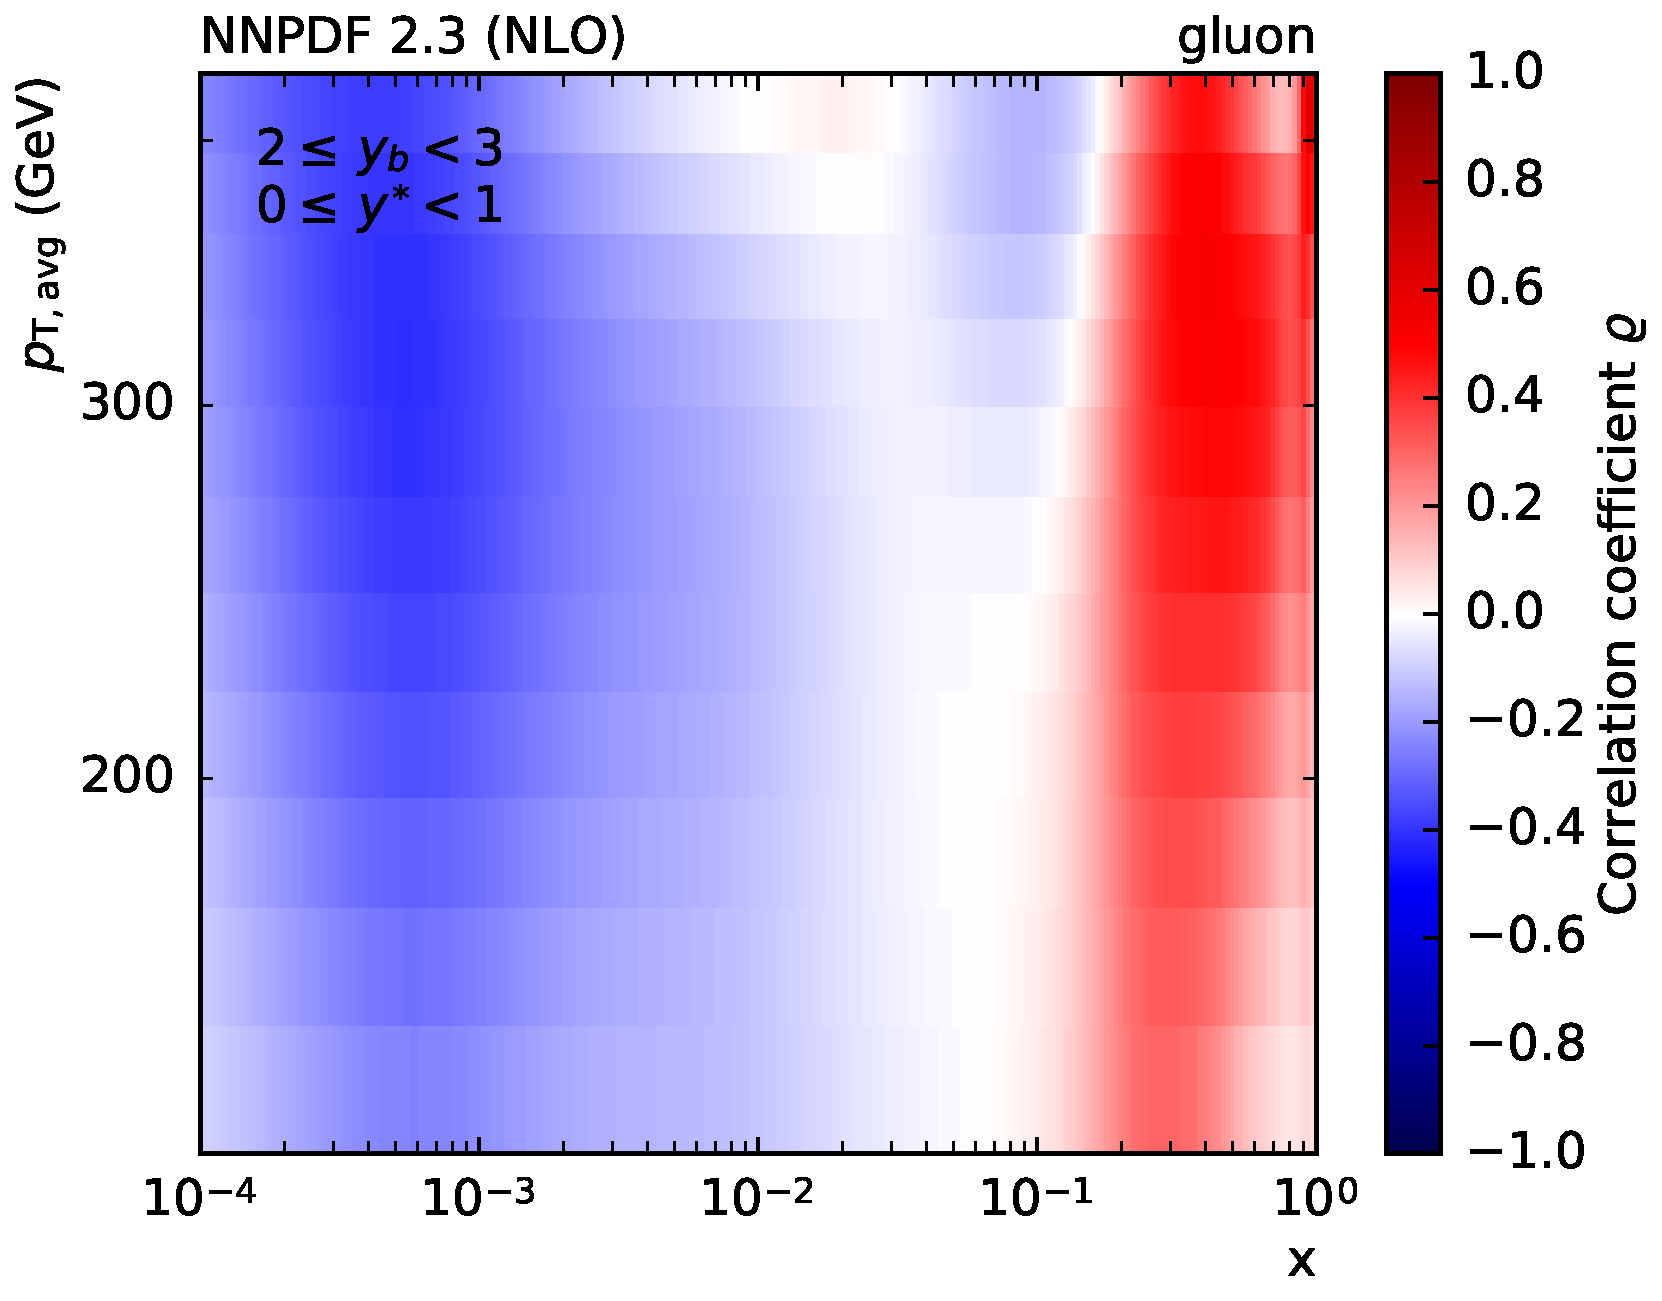
\includegraphics[width=0.49\textwidth]{figures/pdf_constraints/corr_PTMAXEXPYS_YBYS_NLO_FINALBINS_NNPDF23_gluon_ys0_0yb2_0_cl.pdf}
  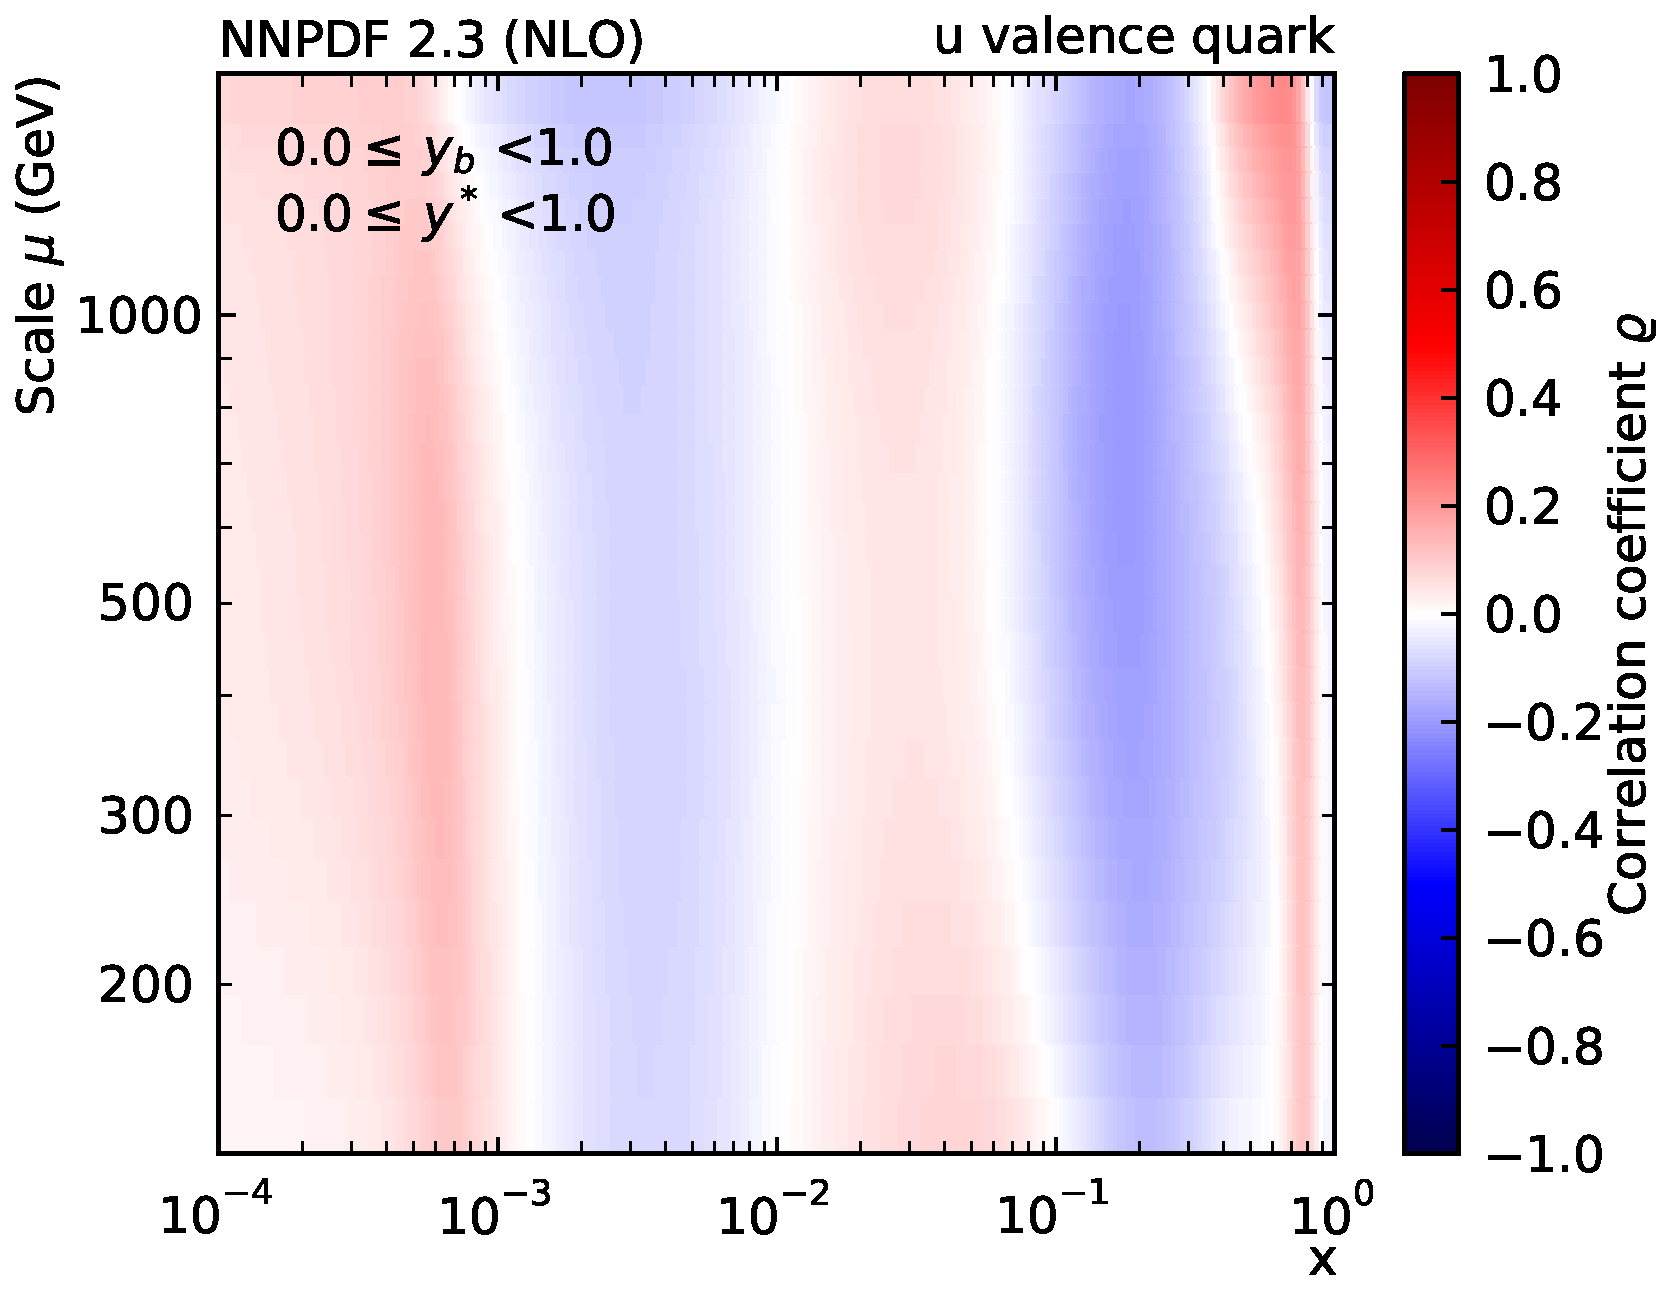
\includegraphics[width=0.49\textwidth]{figures/pdf_constraints/corr_PTMAXEXPYS_YBYS_NLO_FINALBINS_NNPDF23_u_valence_quark_ys0_0yb0_0_cl.pdf}\hfill%
  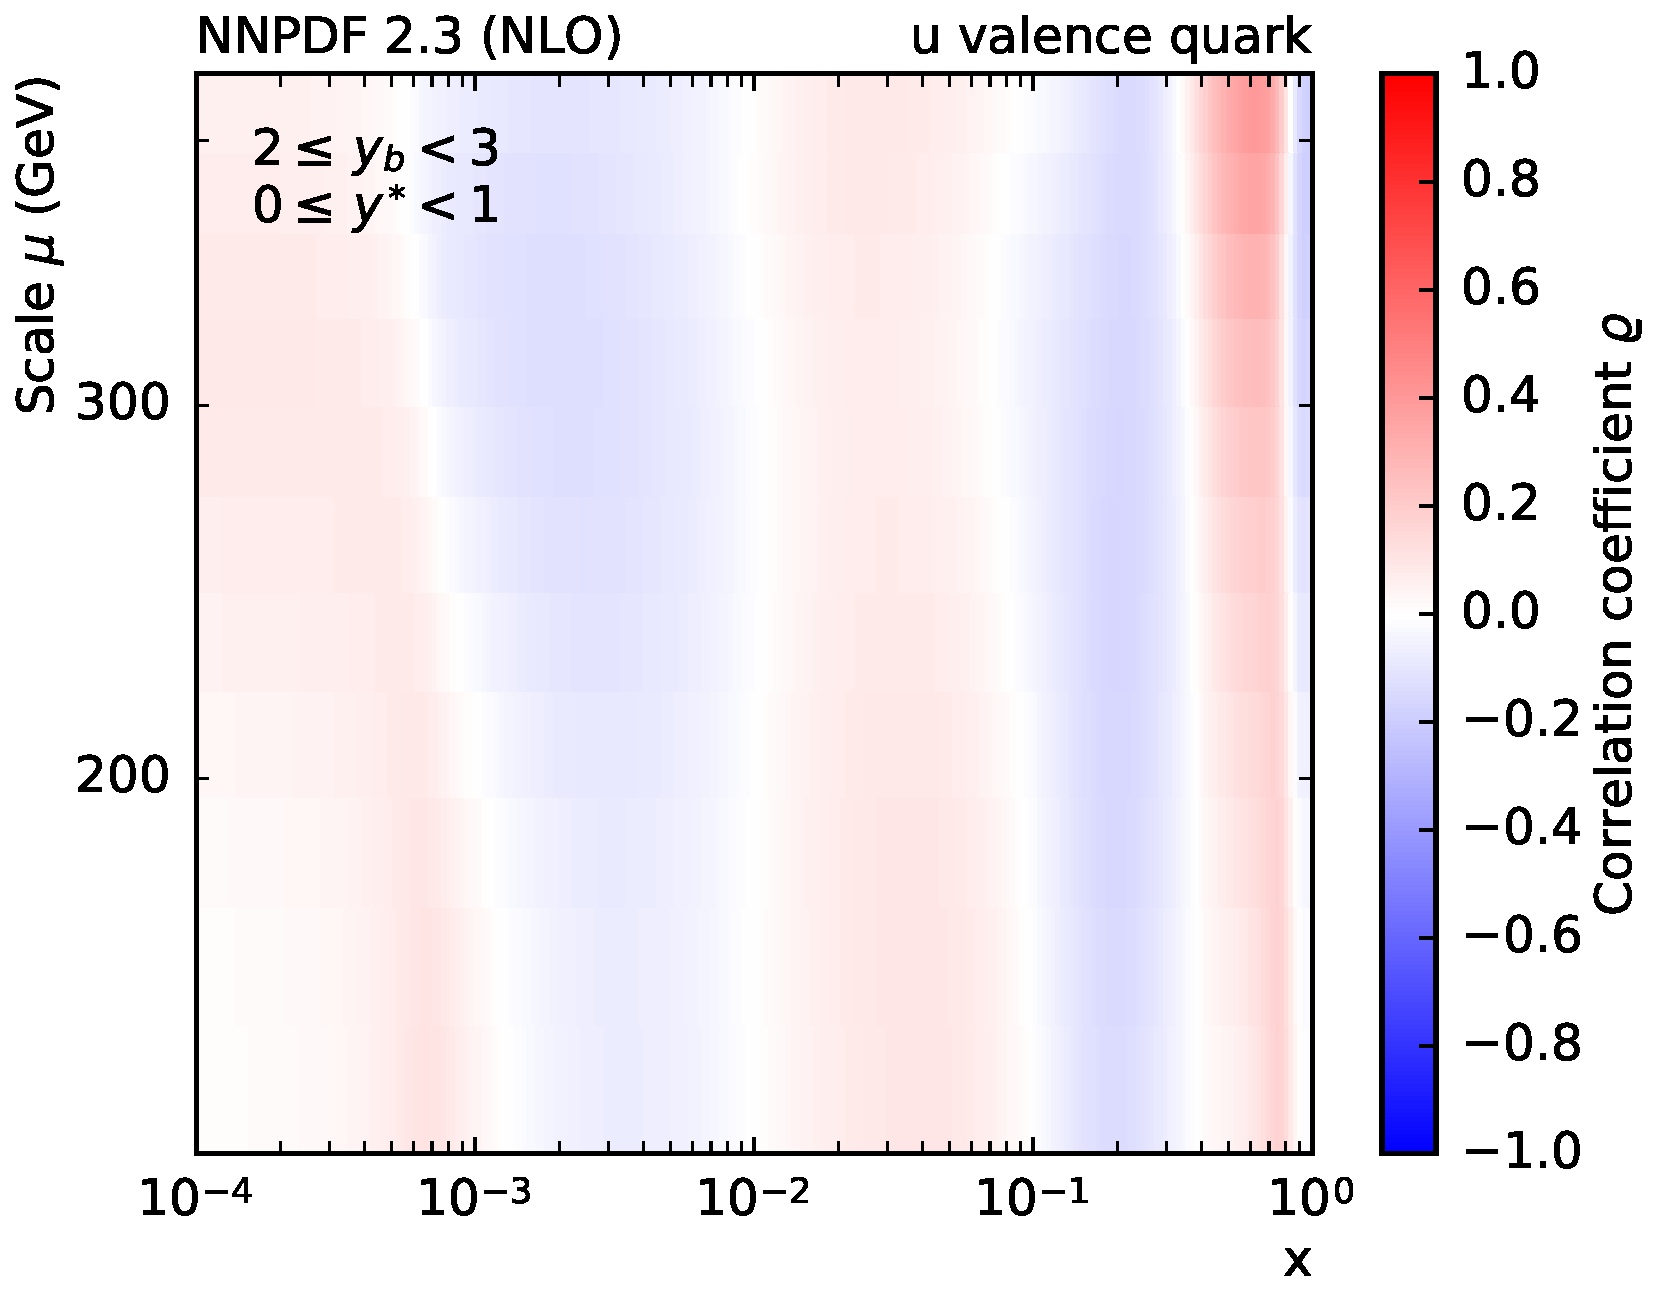
\includegraphics[width=0.49\textwidth]{figures/pdf_constraints/corr_PTMAXEXPYS_YBYS_NLO_FINALBINS_NNPDF23_u_valence_quark_ys0_0yb2_0_cl.pdf}
  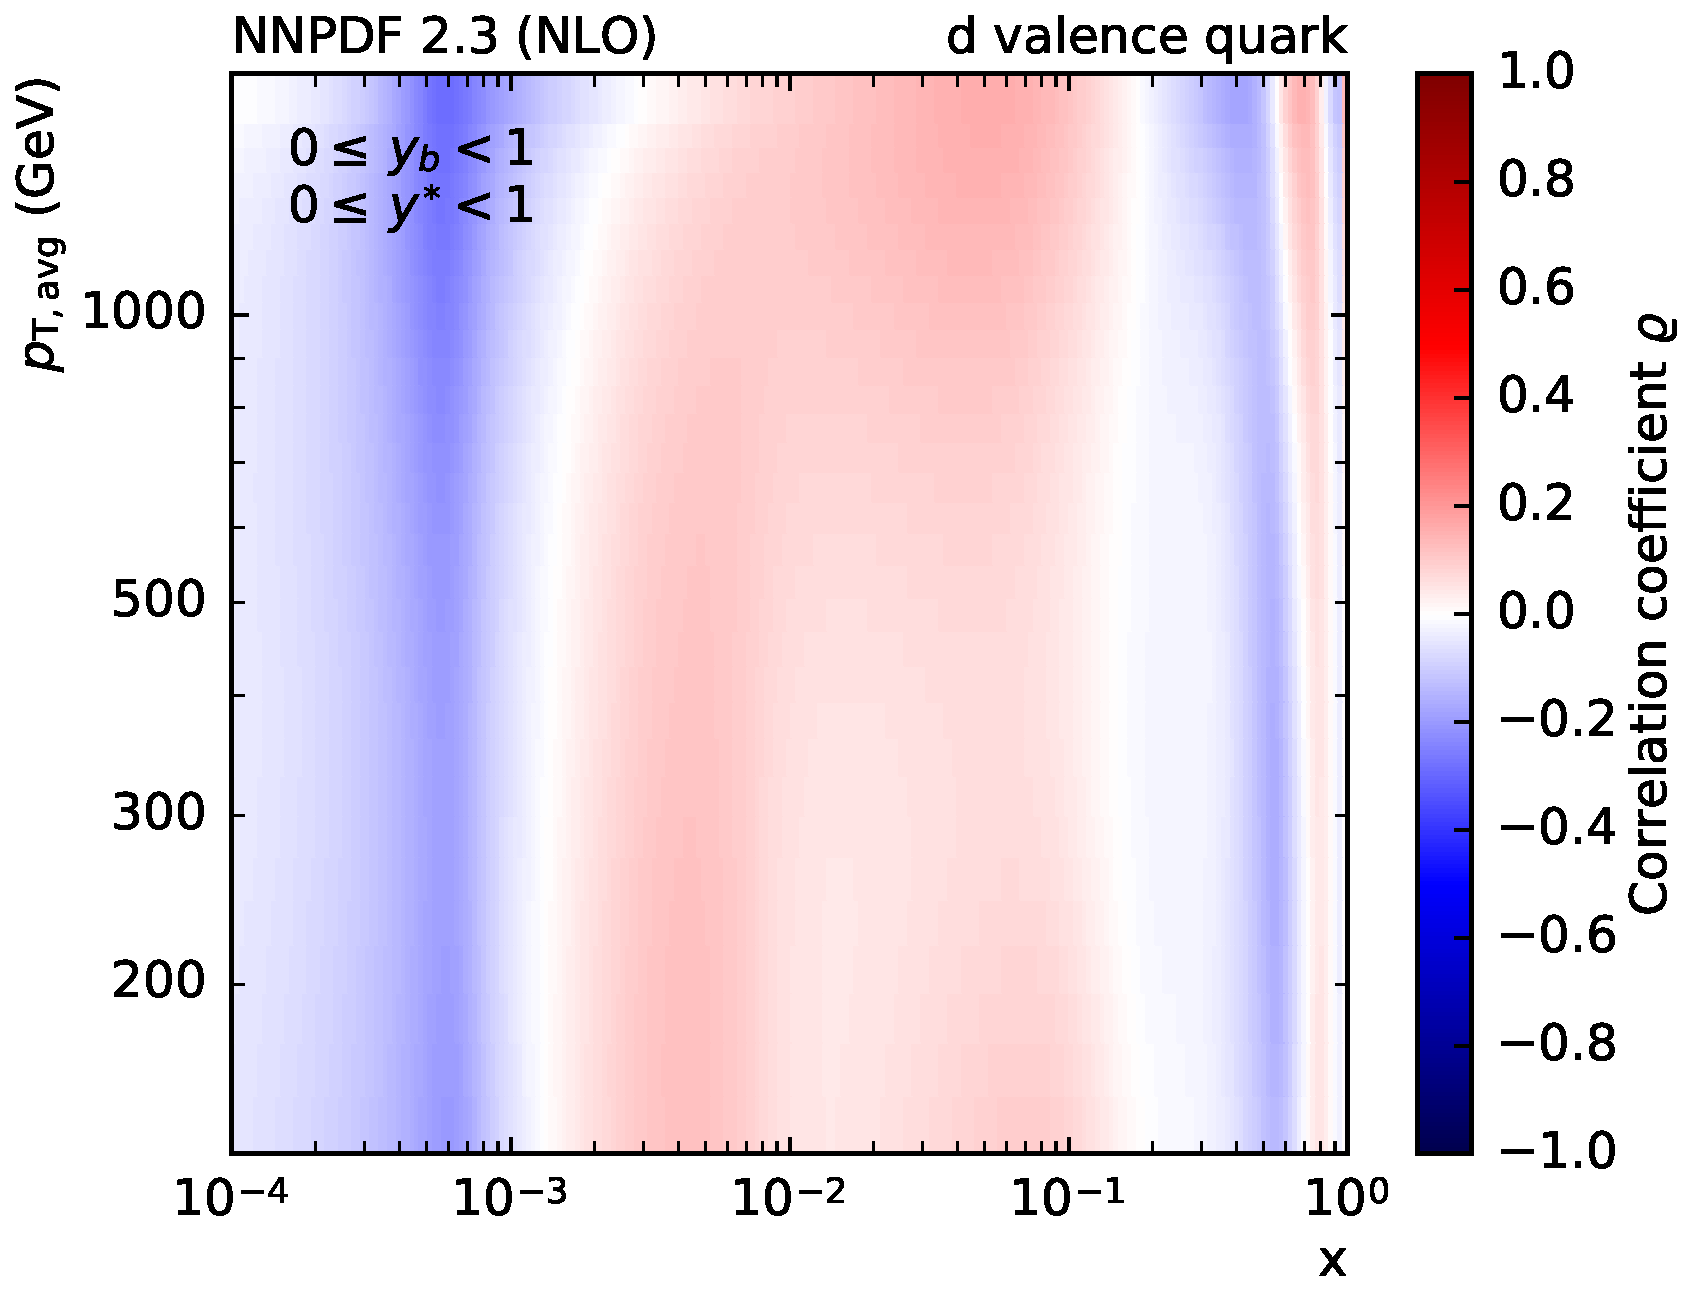
\includegraphics[width=0.49\textwidth]{figures/pdf_constraints/corr_PTMAXEXPYS_YBYS_NLO_FINALBINS_NNPDF23_d_valence_quark_ys0_0yb0_0_cl.pdf}\hfill%
  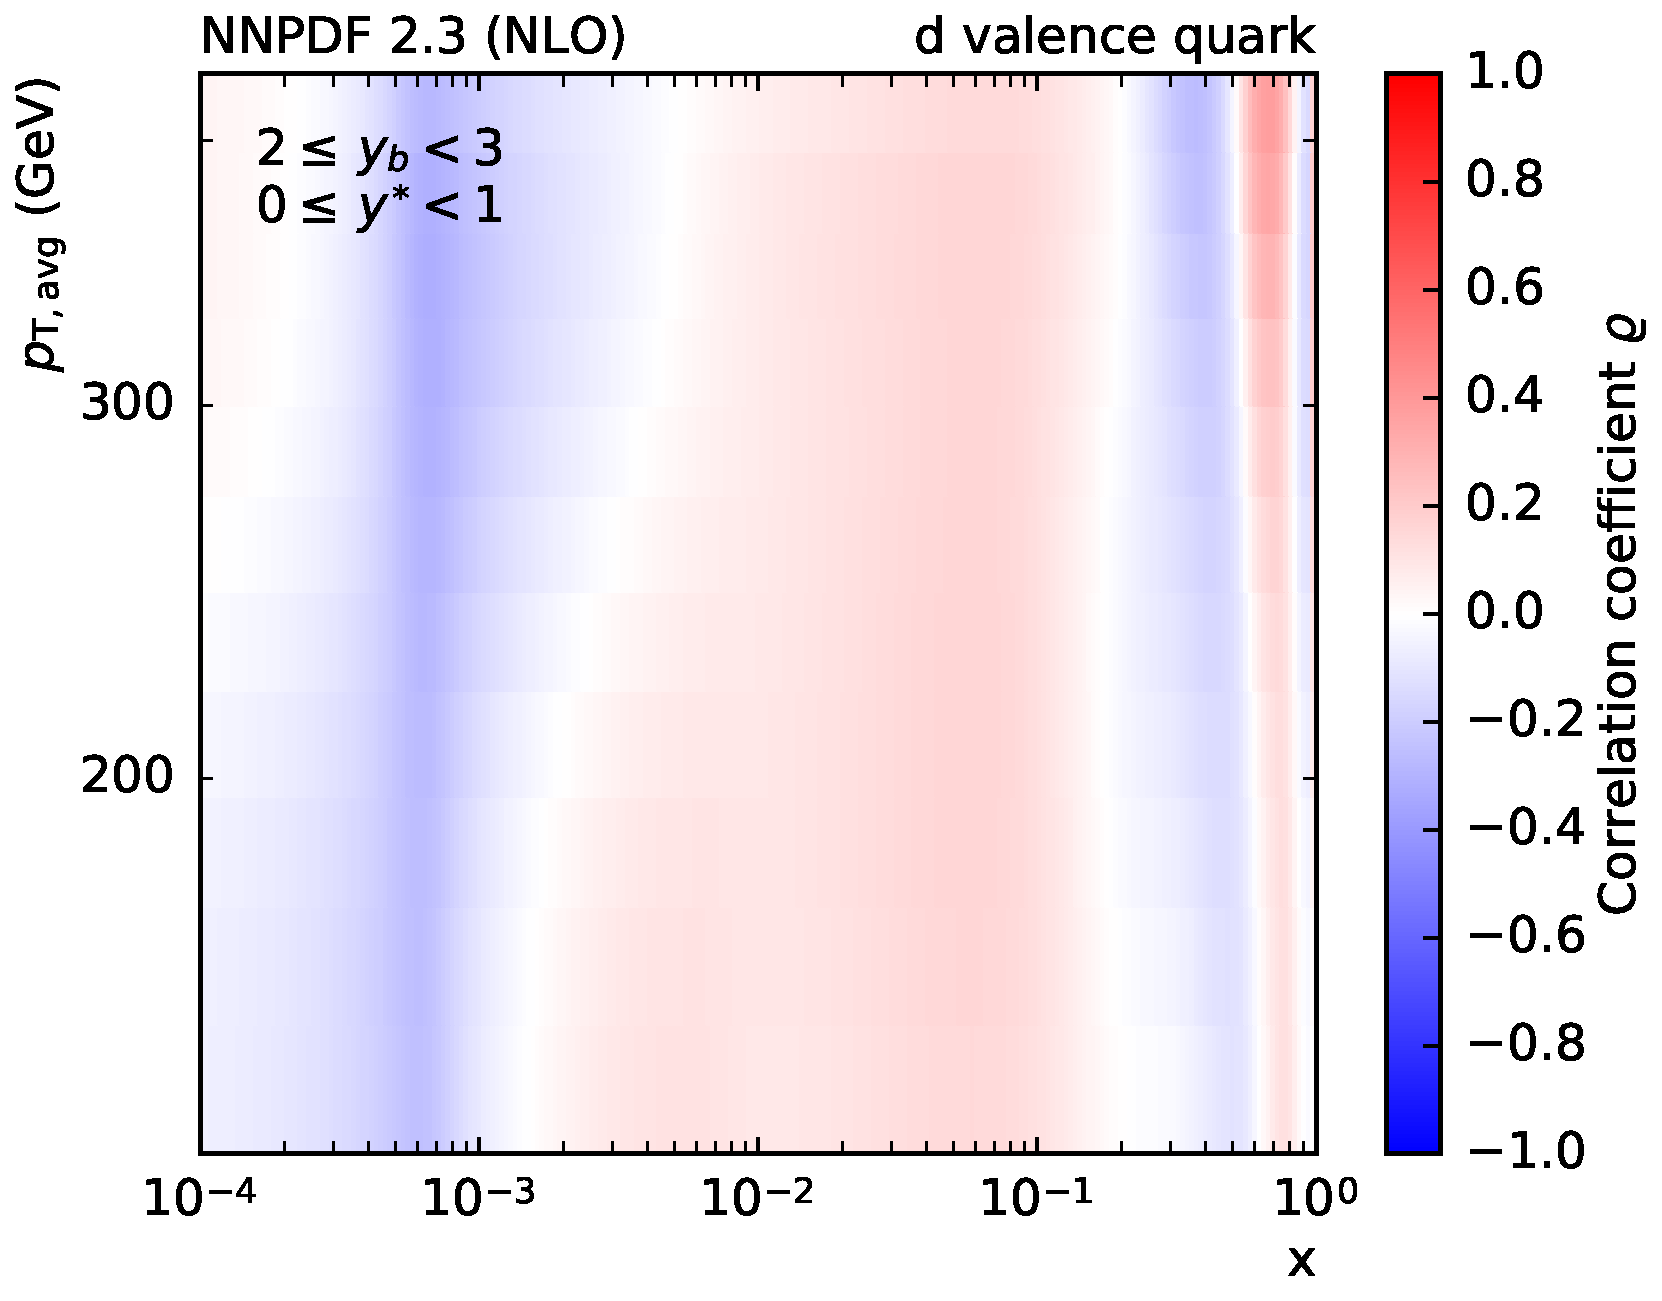
\includegraphics[width=0.49\textwidth]{figures/pdf_constraints/corr_PTMAXEXPYS_YBYS_NLO_FINALBINS_NNPDF23_d_valence_quark_ys0_0yb2_0_cl.pdf}
  \caption{The correlation coefficient between the inclusive jet cross
    section and the gluon (top row), the u valence quark (middle row),
    and the d valence quark PDFs (bottom row), as a function of the
    momentum fraction $x$ of the proton and the energy scale $Q$ of
    the hard process. The correlation is shown for the central
    rapidity region $\yabs<0.5$ (left) and for $2.0<\yabs<2.5$
    (right).}
  \label{fig:correlation_pdf_xs_gqq}
\end{figure}

The correlation between the gluon PDF and the jet cross section is large for
highest \ptavg > \SI{1}{\TeV} and central jets ($\yboost < 1, \ystar < 1$) for
momentum fractions $0.1 < x < 0.5$. In the boosted region ($2 \leq \yboost < 3$)
there is a large correlation for $\SI{200}{\GeV} \leq \ptavg < \SI{400}{\GeV}$
for momentum fractions $0.2 < x < 0.7$. In contrast, the correlation between the
jet cross section and the u valence and d valence quark PDFs is much smaller,
especially in the central region. Again, the correlation for the boosted dijet
region is more pronounced, particularly for highest momentum fractions $x >
0.5$. Based on the results of the correlation studies, a significant impact of
the dijet cross section is expected by including the dijet cross sections in a
PDF fit.

\section{The \xfitter Framework}
\label{section:herafittersetup}

The constraints of the triple-differential dijet measurement on the proton PDFs
is demonstrated by including the cross section measurement in a PDF fit in
combination with inclusive DIS cross sections from the HERA experiments. The
HERA-II DIS data were the basis for the determination of the HERAPDF 2.0 PDF
set.

\xfitter is an open source framework to fit the PDFs to experimental data
based on the Dokshitzer-Gribov-Lipatov-Altarelli-Parisi
(DGLAP)~\cite{Gribov:1972ri,Altarelli:1977zs,Dokshitzer:1977sg} equations. To
ensure consistency between DIS and QCD calculations, the fits are performed at
NLO. The DIS cross sections are calculated by the QCDNUM
software~\cite{Botje:2010ay}.

The parametrization used in the PDF fit is based of the HERAPDF 2.0
parametrization and introduces additional terms which were found to better
describe the additional added jet measurement. The PDFs parameterization is
definded at the starting scale $Q_0$ set to $Q_0 = \SI{1.9}{\GeV \square}$ and
the five independent PDFs $xu_v(x)$, $xd_v(x)$, $xg(x)$, $x\bar{U}(x)$ and
$x\bar{D}(x)$ are parameterized as follows:

\begin{align}
  xg(x) &= A_g x^{B_g} (1-x)^{C_g} (1 + E_g x^2) - A'_g x^{B'_g} (1-x)^{C'_g} \\
  xu_v(x) &= A_{u_{v}} x^{B_{u_{v}}} (1-x)^{C_{u_{v}}}(1 + D_{u_{v}}x + E_{u_{v}}x^2)\\
  xd_v(x) &= A_{d_v} x^{B_{d_v}} (1-x)^{C_{d_{v}}}\\
  x\bar U(x) &= A_{\bar U} x^{B_{\bar U}} (1-x)^{C_{\bar U}}(1 + D_{\bar U}x)\\
  x\bar D(x) &= A_{\bar D} x^{B_{\bar D}} (1-x)^{C_{\bar D}}
\end{align}

Not all parameters are actually fitted. The normalization parameters $A_g$,
$A_{u_{v}}$ and $A_{d_{v}}$ are calculated using the QCD sum rules. $B_{\bar
U}=B_{\bar D}$ and $A_{\bar U} = A_{\bar D}(1-f_s)$ ensure the same
normalization for the $\bar u$ and $\bar d$ PDF for the $x \rightarrow 0$
region. The strangeness fraction is set to $f_s = 0.40$. The generalized-mass
variable flavour number secheme as described in
in~\cite{Thorne:1997ga,Thorne:2006qt} is used with the strong coupling constant
set to $\asmz= 0.1180$.


\subsection{Treatment of Uncertainties in the PDF Fit}
\label{section:treatment_pdf_uncertainties}

The uncertainty of the PDFs is subdivided into three independent sources, which
are evaluated separately and finally added in quadrature to give the total
uncertainty.

\paragraph{Experimental Uncertainties} 
They result from propagated statistical and systematic uncertainties of the data
points and are propagated to the PDF using the Hessian eigenvector
method~\cite{Pumplin:2001ct}. The Hessian matrix is defined by the second
derivatives of the fitted PDF parameters at the \chisq minimum. The matrix is
diagonalized and the eigenvectors are computed, see
Fig.~\ref{fig:eigenvector_basis_set}. 

\begin{figure}[htb]
  \centering
  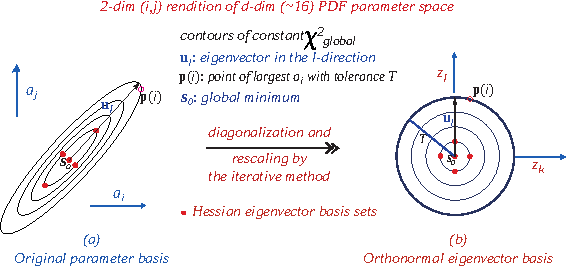
\includegraphics[width=1.0\textwidth]{figures/pdf_constraints/hessianmethod.pdf}
  \caption[Transformation of the parameter basis to the eigenvector basis.]
    {Transformation from the original parameter basis to the orthonormal
    eigenvector basis. The uncertainty on the PDF can be propagated to a
    physical quantity $X$ using these eigenvector PDF sets~\cite{Pumplin:2001ct}.}
    \label{fig:eigenvector_basis_set}
\end{figure}

Using an iterative method, the down- and upwards variation of each eigenvector
corresponding to $\chisq = \chisq_{\mathrm{min}} + 1$ is calculated. Since the
eigenvectors are orthogonal, the eigenvector variation PDFs correspond to
independent sources of uncertainty on the PDFs.

The asymmetric uncertainties $\Delta X^+$ and $\Delta X^-$ on a quantity of
interest $X$ is evaluated as

\begin{align*}
  \Delta X^+_{\mathrm{exp}} &= \sqrt{\sum_i^{N_{\mathrm{EV}}} \left[ \max(X_i^{\mathrm{up}}
    -X_0, X_i^{\mathrm{dn}} - X_0, 0)\right]^2}\\
    \Delta X^-_{\mathrm{exp}} &= \sqrt{\sum_i^{N_{\mathrm{EV}}} \left[ \min(X_i^{\mathrm{up}} - X_0, X_i^{\mathrm{dn}} - X_0,0)\right]^2}
\end{align*}

with $X_0$ describing the central prediction and $X_i^{\mathrm{up}}$ and
$X_i^{\mathrm{dn}}$ giving the quantity using the up- and downwards variation of
the eigenvector PDF set $i$ of the total number of eigenvectors
$N_{\mathrm{EV}}$ in the PDF set.


\paragraph{Model uncertainties} The uncertainties of several parameters input in
the PDF fits are condensed in one PDF model uncertainty. For the model
uncertainties the following variations on the input parameters are considered:

\begin{itemize}
\item The assumption is made, that the shape of the strange PDF follows the
  shape of the fitted down-like sea quarks. Though the strange quark PDF is not
  fitted but determined as a fraction of $xD$ PDF.The strangeness fraction
  $f_s$, by default equal to $0.40$, is varied between $0.30$ and $0.50$.
  \item The b-quark mass is set to $\SI{4.5}{\GeV}$ and varied between
  $\SI{4.25}{\GeV}$ and $\SI{4.75}{\GeV}$.
  \item The c-quark mass, set by default to $\SI{1.47}{\GeV}$ and varied between
  $\SI{1.41}{\GeV}$ and $\SI{1.53}{\GeV}$.
  \item The minimum $Q^2$ value for data used in the fit,
    $Q^2_\mathrm{min}=\SI{7.5}{\GeVsq}$, is varied to $Q^2_\mathrm{min} =
    \SI{5.0}{\GeV\square}$ and $Q^2_\mathrm{min} = \SI{10.0}{\GeV\square}$.
\end{itemize}

The uncertainties are evaluated similar to the eigenvector PDF uncertainties.
The variation of each input parameter is treated as an independent variation.

\begin{align*}
  \Delta X^+_{\mathrm{mod}} &= \sqrt{\sum_i^{N_{\mathrm{N_{\mathrm{par}}}}} \left[ \max(X_i^{\mathrm{up}}
    -X_0, X_i^{\mathrm{dn}} - X_0, 0)\right]^2}\\
    \Delta X^-_{\mathrm{mod}} &= \sqrt{\sum_i^{N_{\mathrm{N_{\mathrm{par}}}}} \left[ \min(X_i^{\mathrm{up}} - X_0, X_i^{\mathrm{dn}} - X_0,0)\right]^2}
\end{align*}

\paragraph{Parameterization uncertainty}

To estimate the influence of the chosen PDF parameterization on the outcome, a
more general form of parametrization is used. Using the general parametrization
for the gluon PDF $xg(x)$ and the quark PDFs $xf(x)$

\begin{align}
   xg(x) &= A_g x^{B_g} (1-x)^{C_g} (1  + D_g x + E_g x^2) - A'_g x^{B'_g} (1-x)^{C'_g};\\
   xf(x) &= A_{f}  x^{B_{f}} (1-x)^{C_{f}} (1 + D_{f}x + E_{f}x^2)
\end{align}

it is studied if the inclusion of additional parameters in the fit yields a
different result. Each parameter is succesively added in the PDF fit and the
envelope of all changes to the PDF shape is collected in a parmeterization
uncertainty. Furthermore the variation of the starting scale $Q_0^2 =
\SI{1.9}{\GeV}$ from \SI{1.6}{\GeV}$ to \SI{2.2}{\GeV}$ is treated as
parametrization uncertainty.

\begin{align*}
  \Delta X^+_{\mathrm{par}} &= \max_{i}^{n} \left[ X^i - X^0, 0 \right]\\
  \Delta X^-_{\mathrm{par}} &= \max_{i}^{n} \left[ X^0 - X^i, 0 \right]
\end{align*}


\subsection{Definition of the goodness-of-fit estimator}
\label{sec:chi2_definition}

The minimization of the PDF fit is using a least-squares method. The \chisq is
calculated with the data points $D_i$ and the theoretical prediction $T_i$. All
$K$ correlated systematic uncertainties $\beta_k$ are treated using nuisance
parameters $r_k$ in a multiplicative way to avoid the bias that arises from data
uncertainties, see~\cite{Lyons:1989gh}. The \chisq is defined as

\begin{equation}
  \chi^2 = \sum_{ij}^N \left(D_i - T_i - \sum_k^K r_k \beta_{ik}\right) \mathrm{C}_{ij}^{-1}
  \left(D_j - T_j - \sum_k^K r_k \beta_{jk} \right) + \sum_k^K r_k^2\,,
  \label{chi2_nuisance}
\end{equation}


\subsection{Treatment of CMS data uncertainties}
\label{section:cmsdatauncertainties}

The dominant source of experimental uncertainty is due to the jet energy scale.
The uncertainty is split into 25 mutually independent sources which are fully
correlated among themselves. 

Since the correlated sources of uncertainty are treated using nuisance
parameters in the \chisq formula, the pull of each source on the fit result can
be examined. Tab.~\ref{tab:pdfconstraints:nuisance} show the 27 sources of
systematic uncertainty and their pulls. Most of the systematic sources shift by
less than one standard deviation $\sigma$ as expected.

\begin{table}[htbp]
  \caption[Nuisance parameters determined in PDF fit]{Nuisance parameters
  obtained by the PDF fit to HERA-I+II DIS data and the CMS dijet cross
  sections. Most of the pulls cause shifts by less than a standard deviation}
  \label{tab:pdfconstraints:nuisance}
  \centering
  \begin{tabular}{lrlr}
    \toprule
    Systematic source        & Shift in $\sigma$ & Systematic source        & Shift in $\sigma$\rbthm\\\midrule
    \textsc{AbsoluteScale}   & -0.18             & \textsc{RelativeFSR}     & 2.45  \rbtrr\\
    \textsc{AbsoluteStat}    & -0.37             & \textsc{RelativeStatEC2} & -0.38  \rbtrr\\
    \textsc{AbsoluteMPFBias} & -0.21             & \textsc{RelativeStatHF}  & 0.03  \rbtrr\\
    \textsc{Fragmentation}   & -0.06             & \textsc{RelativeStatFSR} & -0.06  \rbtrr\\
    \textsc{SinglePionECAL}  & 0.13              & \textsc{PileUpDataMC}    & -0.03  \rbtrr\\
    \textsc{SinglePionHCAL}  & -0.85             & \textsc{PileUpPtRef}     & -1.05  \rbtrr\\
    \textsc{FlavorQCD}       & 1.26              & \textsc{PileUpPtBB}      & 0.89  \rbtrr\\
    \textsc{RelativeJEREC1}  & 0.54              & \textsc{PileUpPtEC1}     & -0.73  \rbtrr\\
    \textsc{RelativeJEREC2}  & -0.26             & \textsc{PileUpPtEC2}     & 0.03  \rbtrr\\
    \textsc{RelativeJERHF}   & 0.04              & \textsc{PileUpPtHF}      & 0.00  \rbtrr\\
    \textsc{RelativePtBB}    & -0.14             & \textsc{nperr}           & -2.02  \rbtrr\\
    \textsc{RelativePtEC1}   & -1.03             & \textsc{jererr}          & 0.36  \rbtrr\\
    \textsc{RelativePtEC2}   & -2.49             & \textsc{lumi}            & 0.62  \rbtrr\\
    \textsc{RelativePtHF}    & 0.01              &                          & \rbtrr\\
    \bottomrule
  \end{tabular}
\end{table}

\section{Constraints on PDFs of the Triple-Differential Dijet Cross Section}
\label{section:cmsjets2011_pdfconstraints}

The quality of the fit with and without including the dijet measurement is
reported in Table~\ref{tab:fit:results}. The partial \chisq per data point for
each dataset as well the \chisq per \ndof for all datasets demonstrate
the compatibility of the CMS dijet measurement and the DIS data from the HERA
experiments. 

\begin{table}[htbp]
\small
\setlength\tabcolsep{3.5pt} 
  \caption[Fit quality in the HERA DIS and combined fit]{The Partial \chisq's  for each dataset in the HERA DIS (middle
    section) or the combined fit including the triple-differential dijet data
    (right section) are shown.
    \ndata is the number of data points available for the determination of
    the 13 parameters. The bottom two lines show the total \chisq and
    \chisqndof. The difference between the sum of all
    \chipsq and the total \chisq for the combined fit is attributed to
    the nuisance parameters.}
  \label{tab:fit:results}
  \centering
  \begin{tabular}{lrrcrc}
    \toprule
    \multicolumn{2}{c}{} &
    \multicolumn{2}{c}{HERA data} &
    \multicolumn{2}{c}{HERA \& CMS data}\rbtrr\\\cmidrule(l){3-6}
    data set &
    \multicolumn{1}{c}{\ndata} &
    \multicolumn{1}{c}{\chipsq} &
    \multicolumn{1}{c}{\chipsqndata} &
    \multicolumn{1}{c}{\chipsq} &
    \multicolumn{1}{c}{\chipsqndata}\rbthm\\\midrule
    CC HERA-I+II H1-ZEUS e-p.                                   & 42  & 54.96  & 1.31  & 54.8   & 1.30 \rbtrr\\
    CC HERA-I+II H1-ZEUS e+p.                                   & 39  & 38.36  & 0.98  & 38.16  & 0.98 \rbtrr\\
    NC HERA-I+II H1-ZEUS e-p.                                   & 159 & 218.2  & 1.37  & 218.99 & 1.38 \rbtrr\\
    NC HERA-I+II H1-ZEUS e+p. $E_{\mathrm{p}} = \SI{460}{\GeV}$ & 187 & 206.83 & 1.11  & 207.62 & 1.11 \rbtrr\\
    NC HERA-I+II H1-ZEUS e+p. $E_{\mathrm{p}} = \SI{575}{\GeV}$ & 234 & 200.8  & 0.86  & 203.07 & 0.87 \rbtrr\\
    NC HERA-I+II H1-ZEUS e+p. $E_{\mathrm{p}} = \SI{820}{\GeV}$ & 63  & 61.14  & 0.97  & 62.73  & 1.00 \rbtrr\\
    NC HERA-I+II H1-ZEUS e+p. $E_{\mathrm{p}} = \SI{920}{\GeV}$ & 332 & 370.18 & 1.12  & 387.34 & 1.17 \rbtrr\\
    CMS Triple-Differential Dijets                              & 111 & ---    & ---   & 90.57  & 0.82
    \rbtrr\\\bottomrule
    data set(s) & \ndof &
    \multicolumn{1}{c}{\chisq} &
    \multicolumn{1}{c}{\chisqndof} &
    \multicolumn{1}{c}{\chisq} &
    \multicolumn{1}{c}{\chisqndof}\rbthm\\\midrule
    HERA data                       & 1042 & 1203.86 & 1.16  &  --- &  --- \rbtrr\\
    HERA \& CMS data                & 1164 &    --- &  --- & 1330.61 & 1.15 \rbtrr\\
    \bottomrule
  \end{tabular}
\end{table}

The resulting PDF for the gluon, u valence, d valence and sea quark PDF are
arranged next to each other in the
Figs.~\ref{fig:pdfconstraints:split:gluonqsea:19}--\ref{fig:pdfconstraints:split:dvaluval:19}
while Fig.~\ref{fig:pdfconstraints:direct:19} and
Fig.~\ref{fig:pdfconstraints:direct:10000} give a direct comparison of the PDFs
with total uncertainties. The fit quality reported in
Table~\ref{tab:fit:results} shows that both HERA DIS and CMS dijet data are
compatible in a combined fit. The uncertainty breakdown in
Fig.~~\ref{fig:pdfconstraints:split:gluonqsea:19} reveals the large impact of
the the dijet data. The uncertainty of the gluon PDF is reduced over almost the
whole range in $x$. The experimental uncertainty is drastically reduced in the
high-$x$ region above $x \gtrsim 0.1$. Less pronounced changes are visible in
the low-$x$ gluon PDF in which most of the uncertainty changes can be attributed
to the parameterization uncertainty. The large changes of uncertainties come
along with a noticeably change of the high-$x$ gluon PDF shape. The gluon PDF is
much harder compared to the fit with HERA DIS data alone. These changes were
observed before, \eg in~\cite{Khachatryan:2014waa}, but are even more pronounced
in this study.

The changes of the sea quark PDF, defined as $asdf$, are much less pronounced.
Only the parametertrization uncertainty is clearly lower in the high-$x$ region.
The u valence and d valence quark PDFs also show uncertainty reductions over
the whole $x$-range. The uncertainty decrease of the experimental uncertainty is
sizable for high-$x$, while the main differences result from the parametrization
uncertainty, which is signifcant for the fit with HERA DIS data alone, but
almost completely vanishes in the fit including the CMS dijet data.

Unlike all previous figures, Fig.~\ref{fig:pdfconstraints:direct:10000} shows
the PDFs after evolution to scale $Q^2 = \SI{10000}{\GeV \square}$. The PDFs
exhibit the same features compared to the starting scale $Q_0$. Finally, an
overview of of the gluon, sea, u valence and d valence quark PDFs is given in
Fig.~\ref{fig:pdfconstraints:overview:19}.   

\begin{figure}[tbp]
  \centering
  \includegraphics[width=0.48\textwidth]{figures/pdf_constraints/hftd/HFTD_HERA_V101_EIG/pdfratio/HFTD_HERA_V101_EIG_0_1_9.pdf}\hfill%
  \includegraphics[width=0.48\textwidth]{figures/pdf_constraints/hftd/HFTD_HERACMSTDJETS_V101_EIG/pdfratio/HFTD_HERACMSTDJETS_V101_EIG_0_1_9.pdf}
  \includegraphics[width=0.48\textwidth]{figures/pdf_constraints/hftd/HFTD_HERA_V101_EIG/pdfratio/HFTD_HERA_V101_EIG_9_1_9.pdf}\hfill%
  \includegraphics[width=0.48\textwidth]{figures/pdf_constraints/hftd/HFTD_HERACMSTDJETS_V101_EIG/pdfratio/HFTD_HERACMSTDJETS_V101_EIG_9_1_9.pdf}
  \caption[The gluon and sea quark PDFs]{The gluon (top) and sea quark (bottom) PDFs as a function of $x$ as
  derived from HERA-II inclusive DIS data alone (left) and in combination with
  the CMS dijet data (right). The PDFs are shown at the starting scale $Q^2 =
  \SI{1.9}{\GeV \square}$. The experimental (inner band), model (middle band)
  and parameterization uncertainties (outer band) are added quadratically to give
  te total uncertainty.}
  \label{fig:pdfconstraints:split:gluonqsea:19}
\end{figure}

\begin{figure}[tbp]
  \centering
  \includegraphics[width=0.48\textwidth]{figures/pdf_constraints/hftd/HFTD_HERA_V101_EIG/pdfratio/HFTD_HERA_V101_EIG_7_1_9.pdf}\hfill%
  \includegraphics[width=0.48\textwidth]{figures/pdf_constraints/hftd/HFTD_HERACMSTDJETS_V101_EIG/pdfratio/HFTD_HERACMSTDJETS_V101_EIG_7_1_9.pdf}
  \includegraphics[width=0.48\textwidth]{figures/pdf_constraints/hftd/HFTD_HERA_V101_EIG/pdfratio/HFTD_HERA_V101_EIG_8_1_9.pdf}\hfill%
  \includegraphics[width=0.48\textwidth]{figures/pdf_constraints/hftd/HFTD_HERACMSTDJETS_V101_EIG/pdfratio/HFTD_HERACMSTDJETS_V101_EIG_8_1_9.pdf}
  \caption[The d valence and u valence quark PDFs]{The d valence quark (top) and u
    valence quark (bottom) PDFs as a function of $x$ as
  derived from HERA-II inclusive DIS data alone (left) and in combination with
  the CMS dijet data (right). The PDFs are shown at the starting scale $Q^2 =
  \SI{1.9}{\GeV \square}$. The experimental (inner band), model (middle band)
  and parameterization uncertainties (outer band) are added quadratically to give
  te total uncertainty.}
  \label{fig:pdfconstraints:split:dvaluval:19}
\end{figure}


\begin{figure}[tbp]
  \centering
  \includegraphics[width=0.48\textwidth]{figures/pdf_constraints/hftd/direct/HFTD_HERACMSTDJETS_V101_EIG/pdfratio/HFTD_HERACMSTDJETS_V101_EIG_0_1_9.pdf}\hfill%
  \includegraphics[width=0.48\textwidth]{figures/pdf_constraints/hftd/direct/HFTD_HERACMSTDJETS_V101_EIG/pdfratio/HFTD_HERACMSTDJETS_V101_EIG_9_1_9.pdf}
  \includegraphics[width=0.48\textwidth]{figures/pdf_constraints/hftd/direct/HFTD_HERACMSTDJETS_V101_EIG/pdfratio/HFTD_HERACMSTDJETS_V101_EIG_7_1_9.pdf}\hfill%
  \includegraphics[width=0.48\textwidth]{figures/pdf_constraints/hftd/direct/HFTD_HERACMSTDJETS_V101_EIG/pdfratio/HFTD_HERACMSTDJETS_V101_EIG_8_1_9.pdf}
  \caption[Direct comparison of gluon and quark PDFs]{The gluon (top left), sea
  quark (top right), d valence quark (bottom left) and u valence quark (bottom
right) PDFs as a function of $x$ as derived from HERA-II inclusive DIS data
alone (dashed line) and in combination with CMS dijet data (full line). The PDFs
are shown at the starting scale $Q^2 = \SI{1.9}{\GeV \square}$. The total
uncertainty of the PDF is shown (hatched and solid bands).}
  \label{fig:pdfconstraints:direct:19}
\end{figure}

\begin{figure}[tbp]
  \centering
  \includegraphics[width=0.48\textwidth]{figures/pdf_constraints/hftd/direct/HFTD_HERACMSTDJETS_V101_EIG/pdfratio/HFTD_HERACMSTDJETS_V101_EIG_0_10000_0.pdf}\hfill%
  \includegraphics[width=0.48\textwidth]{figures/pdf_constraints/hftd/direct/HFTD_HERACMSTDJETS_V101_EIG/pdfratio/HFTD_HERACMSTDJETS_V101_EIG_9_10000_0.pdf}
  \includegraphics[width=0.48\textwidth]{figures/pdf_constraints/hftd/direct/HFTD_HERACMSTDJETS_V101_EIG/pdfratio/HFTD_HERACMSTDJETS_V101_EIG_7_10000_0.pdf}\hfill%
  \includegraphics[width=0.48\textwidth]{figures/pdf_constraints/hftd/direct/HFTD_HERACMSTDJETS_V101_EIG/pdfratio/HFTD_HERACMSTDJETS_V101_EIG_8_10000_0.pdf}
  \caption[Direct comparison of gluon and quark PDFs]{The gluon (top left), sea
  quark (top right), d valence quark (bottom left) and u valence quark (bottom
right) PDFs as a function of $x$ as derived from HERA-II inclusive DIS data
alone (dashed line) and in combination with CMS dijet data (full line). The PDFs
are shown at the starting scale $Q^2 = \SI{10000}{\GeV \square}$. The total
uncertainty of the PDF is shown (hatched and solid bands).}
\label{fig:pdfconstraints:direct:10000}
\end{figure}

\begin{figure}[tbp]
  \centering
  \includegraphics[width=0.9\textwidth]{figures/pdf_constraints/hftd/overview/HFTD_HERACMSTDJETS_V101_EIG/pdfoverview/HFTD_HERACMSTDJETS_V101_EIG_1_9.pdf}\hfill%
  \caption[Overview of gluon and quark PDFs]{Overview of the gluon, sea, u
  valence and d valence quark Pdfs before (dashed line) and after (full line)
  including the CMS dijet data int the fit. The PDFs are shown at the starting
  scale $Q^2 = \SI{1.9}{\GeV \square}$. The total uncertainty including the dijet
  data is shown as solid bind around the central fit result.}
  \label{fig:pdfconstraints:overview:19}
\end{figure}

\section{Simultaneous Fit of PDFs and Strong Coupling}

The triple-differential dijet cross section does not only provide constraints on
the PDFs, but also on the strong coupling constant. The bin which contains the
boosted dijet events is the most sensitive to the PDFs. However, the
experimental uncertainties are larger than in the bin containing two central
jets, \ie at low \yboost and low \ystar values. At the same time, the highest
transverse momentum are reached in that bin. Due to the known correlations
between these phase space regions, this measurement is a good input for a
simultaneous fit of both the PDFs and the strong coupling. 

Therefore, the same PDF fit as in the previous section is performed but with the
additional free parameter \as. The uncertainty on \as is determined using
\textsc{Minuit} by profiling the likelihood. Furthermore, the model and
parameterization uncertainties were calculated in the same way as in
Sec.~\ref{section:cmsjets2011_pdfconstraints}. In addition, the scale
uncertainties are estimated by varying the renormalization and factorization
scale and repeating the fit in a similar way as in
Sec.~\ref{sec:scale_uncertainties}. The scale of the HERA DIS remained
unchanged. 

The strong coupling constant \asmz is determined as

\begin{equation*}
  \asmz = 0.1188_{-0.0015}^{+0.0015}(\mathrm{exp})_{-0.0002}^{+0.0004}(\mathrm{mod})_{-0.0005}^{+0.0003}(\mathrm{par})_{-0.0010}^{+0.0029}(\mathrm{scale})
\end{equation*}

where the \emph{exp} uncertainty accounts for the experimental uncertainties of
the incvlusive HERA DIS and CMS jet data and NP uncertainties. The \emph{mod}
and \emph{par} uncertainty denotes the model respectively the parameterization
uncertainty and \emph{scale} the scale uncertainties.  The determined value of
\asmz in agreement with the world average of $\asmz=0.1181\pm 0.0013$ of the
PDG~\cite{Agashe:2014kda}.
